\addchapheadtotoc
\chapter{Background on Radiation in Combustion}\label{chapter:Importance}

\section{Fundamentals of radiation} \label{Sec:FundOfRad}
The term \textit{radiative heat transfer} commonly refers to the transfer of thermal energy through electromagnetic waves~\cite{Modest2022ChapterRadiation}.
% Thermal radiation is the transfer of thermal energy through electromagnetic waves, according to electromagnetic wave theory, and by particulate photons, according to quantum mechanics~\cite{Modest2013RadiativeTransfer}. 
% Either perspective may be more convenient for a given circumstance, but both perspectives are required for a complete definition \cite{Modest2013RadiativeTransfer}. 
This transfer occurs at the speed of light, which is $2.998 \times 10^8$ meters per second in a vacuum, a speed much higher than what is seen in most combustion processes on earth.
The effects of thermal radiation can be seen in everyday life. Common examples include the sun, a campfire, and a hot pavement. 
Wavelengths range from picometers ($10^{-12}$ m) for gamma rays to megameters ($10^6$ m) for ultra-low frequency radio waves.
For combustion systems, relevant wavelengths generally fall between 1 and 15 $\mu{}$m ($10^{-6}$ m), in the infrared and visible light parts of the electromagnetic spectrum~\cite{Liu2020TheFlames}.

Transport of thermal radiation is known to have a non-local nature. Radiation emitted at one point in space can impact the energy and temperature at another point very far away. 
This is in contrast to conductive and convective modes of heat transfer where thermal energy is transferred through direct contact (local phenomena). 
% It is for this reason that radiation plays a very important role in massive-scale studies such as in the vacuum of space.
Relevant fundamental laws for radiation in combustion systems are briefly reviewed below.
Readers can refer to \cite{Howell2010ThermalTransfer,Modest2013RadiativeTransfer} for more thorough descriptions.

\subsection{Basic laws of radiation}\label{section:BasicLaws}

\subsubsection{The idealized `Black body'}
The term \textit{black body} refers to a theoretical object that can absorb all incident radiation. The term \textit{black} is used because a body that absorbs perfectly does not reflect any light and must therefore appear to be black. In addition, according to arguments posed by Kirchhoff~\cite{Bergman2017FundamentalsTransfer}, black bodies are also ideal emitters.
Black bodies are commonly employed as the perfect emitter and absorbers in radiation calculations in the literature.

The emission spectrum of a black body was derived by Max Planck, and is shown in Eq.~\ref{eq:PlancksLaw},
\begin{equation}
    E_{bv}(T,\nu{}) = \frac{2\pi{}\hbar\nu{}^3n^2}{c_0^2\left[e^\frac{\hbar\nu{}}{kT}-1\right]}\ ,
    \label{eq:PlancksLaw}
\end{equation}
where $\hbar$ is Planck's constant, $\nu{}$ is the wave frequency, $n$ is the refractive index of the medium, $c_0$ is the speed of light in a vacuum, $k$ is the Boltzmann constant, and $T$ is the temperature of the body. The wave frequency can be related to the wavelength $\lambda$ as,
\begin{equation}
    \lambda{}=\frac{c}{\nu}\ ,
    \label{eq:FrequencyToWavelength}
\end{equation}
where $c$ is the speed of light in the medium. When Eq.~\ref{eq:PlancksLaw} is integrated across the electromagnetic spectrum (from $\nu=0$ to $\nu=\infty$), the overall emissive power from the surface of a black body is evaluated as
\begin{equation}
    E_b(T) = n^2\sigma{}T^4\ ,
    \label{eq:PlancksLawIntegrated}
\end{equation}
where emissive power has dimensions of [ power / area on surface ]. 

A more fundamental quantity of radiation is the radiative intensity, $I$, which has dependence on direction and wavelength. Intensity defines the emission in dimensions of [ power / area / unit solid angle / wavelength ]. %where the area is now the unit area normal to the direction of interest as opposed to the unit area on the surface as it is for emissive power. 
A ``solid angle'' is a description of a differential area along the unit sphere, similar to an angle on the unit circle.
% While radians are used as angular units of a unit circle, sterradians are used for angular units along the unit sphere. 

For a black body, intensity has no directional dependence (i.e. is \textit{diffuse}). Black body emissive power can be evaluated from intensity by integrating over the hemispherical solid angle of emission from a surface, as 
\begin{equation}
    E_b(\textbf{r},T) = \int_{2\pi}{I_b(\textbf{r},\hat{\textbf{s}},T)}~d\Omega{}\ ,
    \label{eq:EmissivePowerFromIntensity}
\end{equation}
where the variable of integration, $\Omega{}$, is the solid angle, $\hat{\textbf{s}}$ is direction, and $\textbf{r}$ is the point of interest. The solution of the integration requires accounting for the change in perspective of the unit area on the surface at different angles, and results in
\begin{equation}
    I_b(T) = \frac{E_b(T)}{\pi}\ ,
    \label{eq:Intensity}
\end{equation}
where the subscript $b$ denotes blackbody. 

\subsubsection{Kirchhoff's Law} \label{sec:KirchoffsLaw}
Kirchhoff's law proves that a black-body is both an ideal emitter and absorber and can be described through a simple thought experiment, as follows. Two systems are constructed consisting of an enclosure of black-body surfaces surrounding an object. The object in the first system is a black-body, and the object in the second system is a non-ideal absorber. Both systems are thermally insulated to the surroundings. 
According to the second law of thermodynamics, after a long period of time, the temperatures in both systems will independently equalize to constant values. This implies that the energy emitted and absorbed by the object and the surroundings in each system should be the same.
Kirchhoff postulated that since a black body is a better absorber than the gray body, the second law requires it to be a better emitter. Therefore, because a black-body is the most ideal absorber, it must also be the most ideal emitter of radiation, as this argument applies for any variation of non-ideal absorber.
Further continuation of this argument reveals that the ratio of emission of any object to that of a black body must also equal the ratio of the absorption of that object to that of a black body, and that this argument applies for emission at any wavelength $\eta$ (inverse of $\lambda$) and any direction $\theta$ for in-going or out-going electromagnetic rays. Kirchhoff therefore established the equality of spectral, directional emissivity $\epsilon_{\eta{}\theta{}}$ and spectral, directional absorptivity $\alpha{}_{\eta,\theta}$ at thermal equilibrium, as shown in Eq.~\ref{eq:KirchhoffsLaw},
\begin{equation}
    \epsilon{}_{\eta{}\theta{}}=\alpha{}_{\eta{}\theta{}}\ .
    \label{eq:KirchhoffsLaw}
\end{equation}

\subsection{Spectral effects}\label{Sec:Nongray}
% Unlike a black body, gases emit radiation in a discontinuous manner.
The black body spectrum discussed in section~\ref{section:BasicLaws} can approximate the emission spectrum from the surface of many solid materials, but is discouraged for use with gas emission. 
Most solid structures have a multitude of modes of oscillations, from the crystal-lattice structure down to the molecular energy states~\cite{Viskanta1975HeatSolids}. As a result, the emission spectra of solids are often continuous and can be approximated as a constant fraction of the black body emission spectrum (i.e. gray)~\cite{Howell2010ThermalTransfer}. 
However, gases are restricted to the oscillation modes of the natural energy states of the individual molecules in the mixture. Quantum mechanics postulates that the energy states of molecules are discrete, and therefore the change in energy states and resulting emission spectra are also discrete~\cite{Hanson2016SpectroscopyGases}.
\begin{figure}
\centering
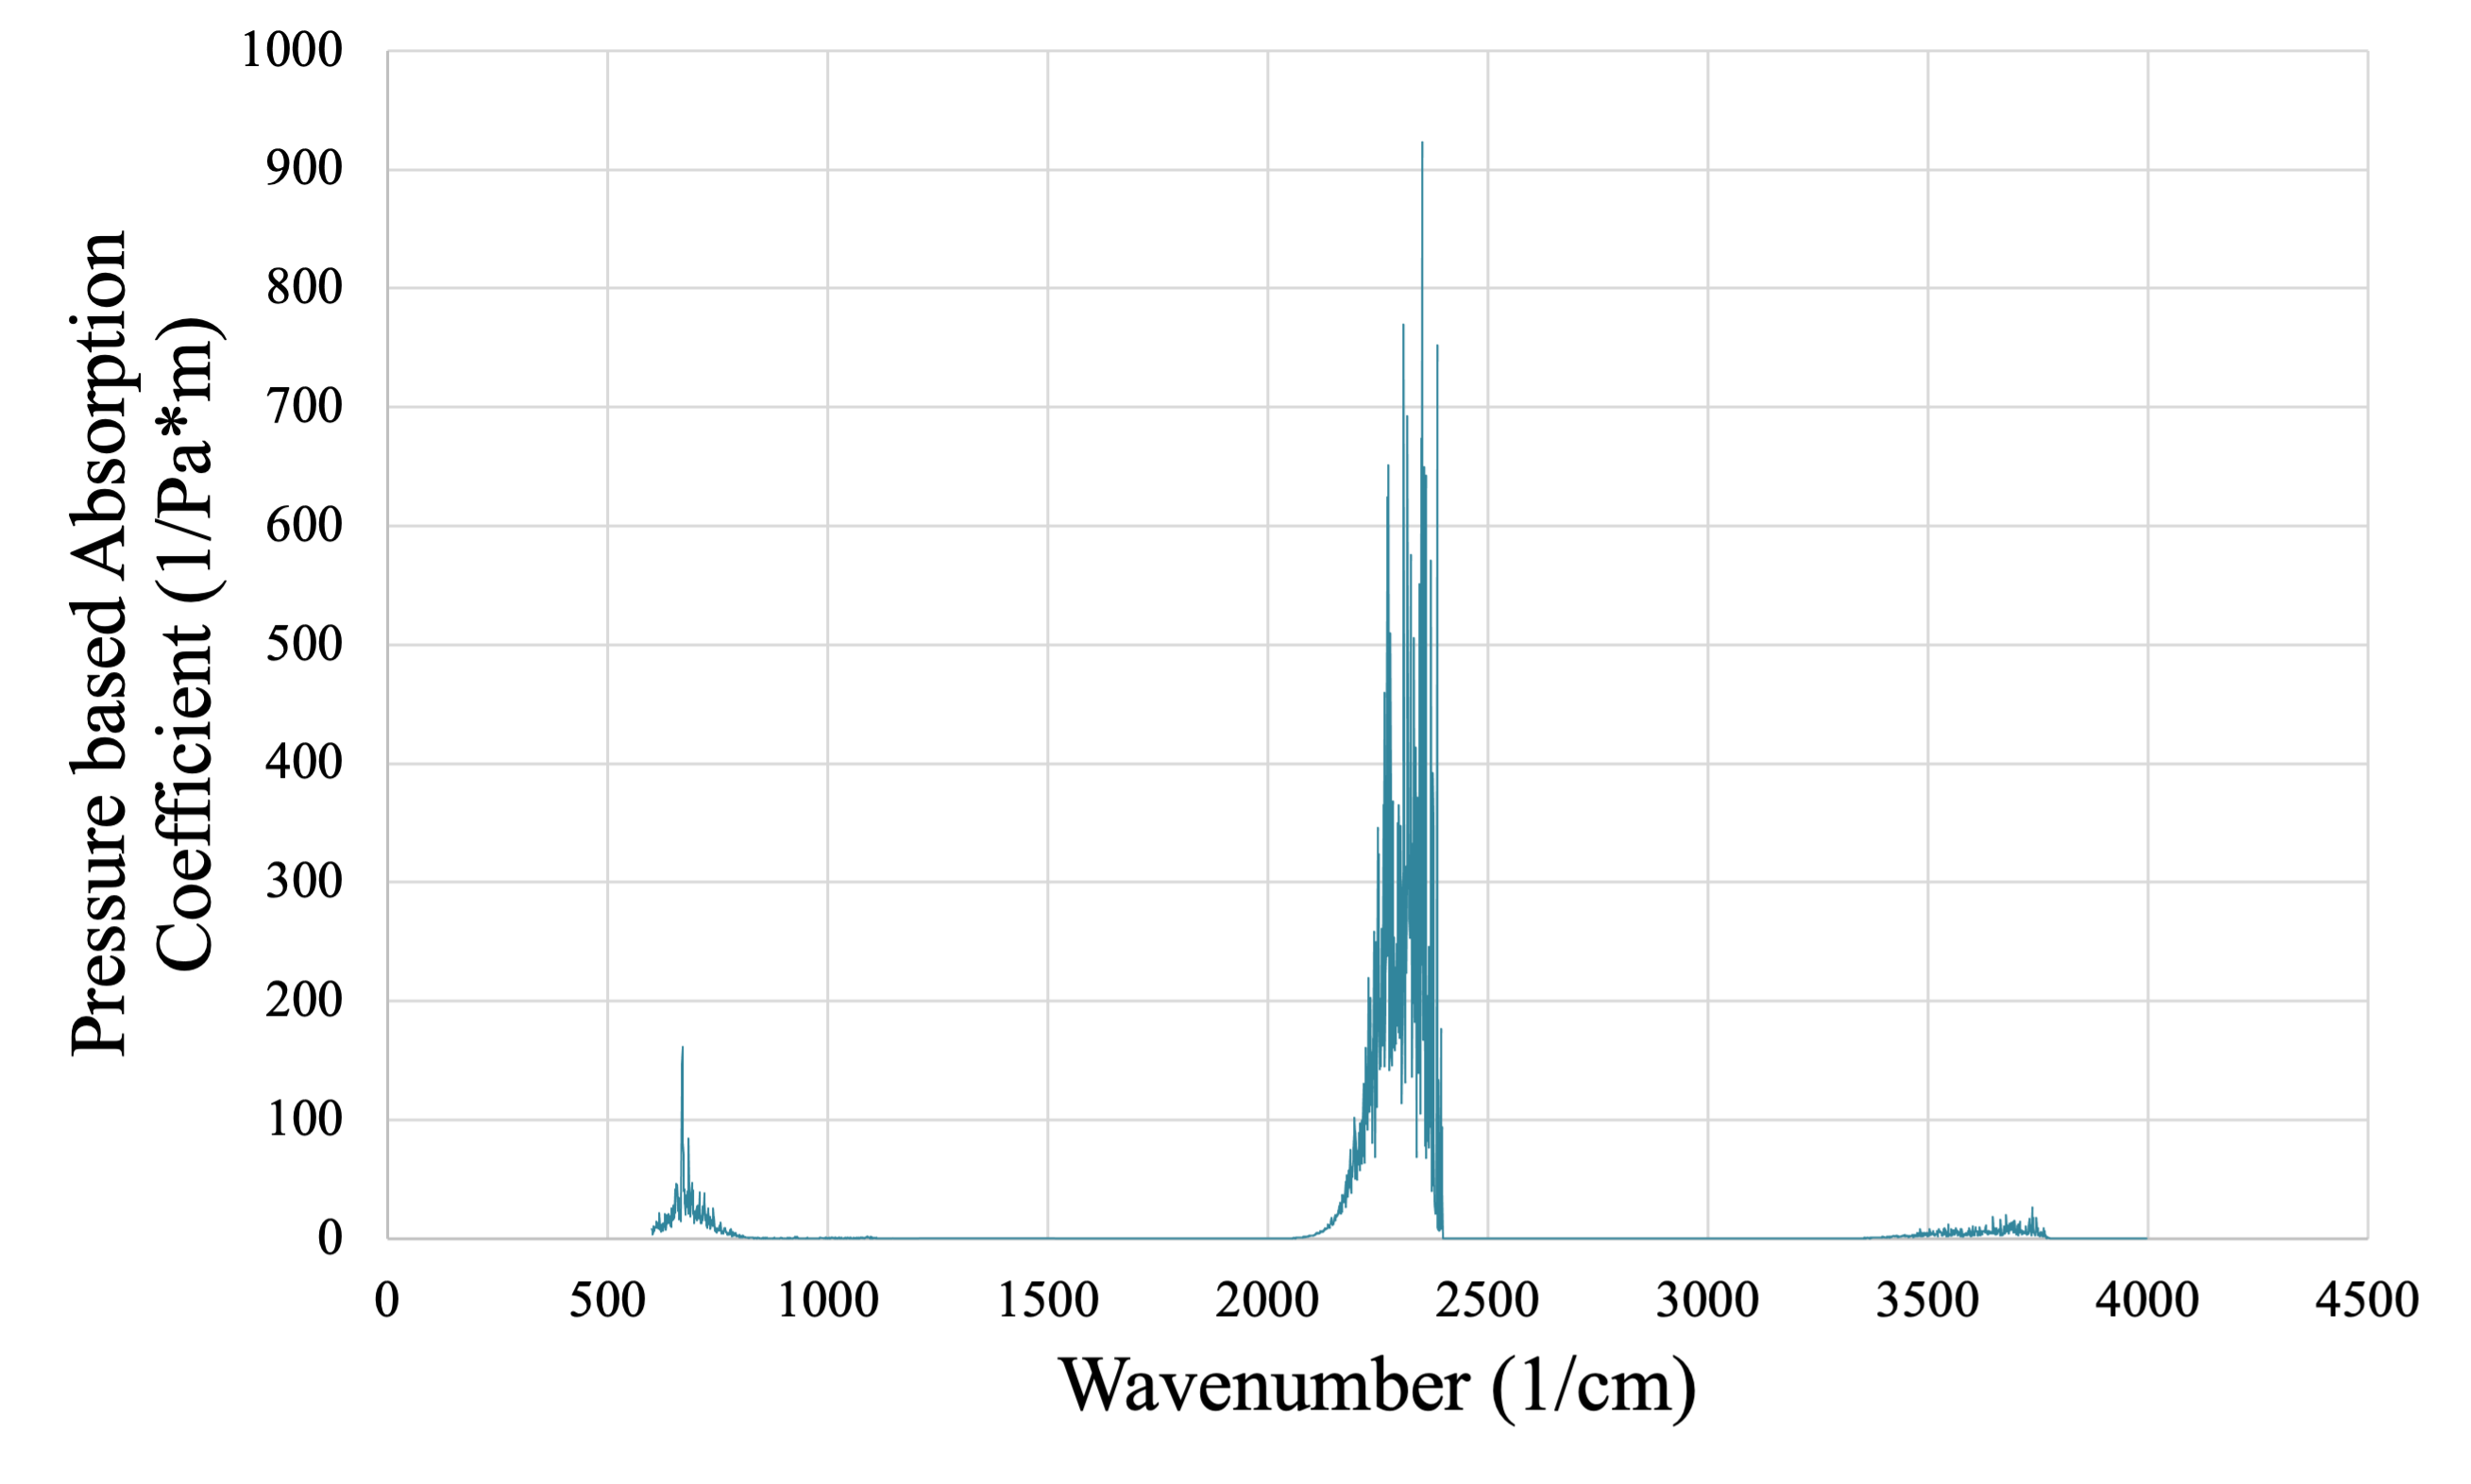
\includegraphics[width=0.8\linewidth]{figures/ch2/SpectralLinesCO2.png}
\caption{Spectrals lines of CO$_2$ at $1$ bar and $1600$ K below 4000 1/cm obtained from a line-by-line database~\cite{Ren2013AGases}.}
\label{fig:SpectralLines}
\end{figure}


The largest molecular contributors to emission in most hydrocarbon flames are CO$_2$, CO, H$_2$O, and soot. Figure~\ref{fig:SpectralLines} shows the absorption coefficient spectrum of CO$_2$~\cite{Liu2020TheFlames}. 
\textit{Ab initio} modeling and experimental data are nowadays used to obtain approximations for the emission spectra of a molecule at a specified pressure and temperature~\cite{Hanson2016SpectroscopyGases}. This information has been collected into a series of online databases such as HITEMP~\cite{Rothman2010HITEMPDatabase}, which are used to predict absorption coefficients for given gaseous thermodynamic states and wavelengths.

Radiation from soot can make the emission spectra of flames much more continuous.
Soot particles are generated through the agglomeration of unburnt hydrocarbons~\cite{Mueller2013LargeCombustor}. The resulting particulates contribute much to the visual yellow glow seen in flames, ergo sooting flames are known as \textit{luminous}. 
Soot particles have sizes of only tens of microns, and volume fractions of order $10^{-4}$\% to $10^{-6}$\%, but often contribute the majority of radiation from a flame when present~\cite{Modest2016RadiativeSystems}.

\subsection{Thermal radiation in participating media} \label{section:RTE}
For combustion systems, thermal radiation interacts with the medium as well as the walls. The governing equation to describe radiation in an absorbing-emitting medium is the radiative transfer equation (RTE), as in Eq.~\ref{eq:RTE2},
\begin{equation}
    \frac{dI_\eta{}}{ds} = \hat{\textbf{s}} \cdot \nabla{I_\eta{}} = \kappa{}_\eta{}I_{b\eta{}}-\kappa{}_\eta{}I_\eta{}-\sigma{}_{s\eta{}}I_\eta{}+\frac{\sigma{}_{s\eta{}}}{4\pi}\int_{4\pi{}}{I_\eta{}(\hat{\textbf{s}})\Phi_\eta{}(\hat{\textbf{s}}_i,\hat{\textbf{s}})}\,d\Omega{}_i \ ,
    \label{eq:RTE2}
\end{equation}
where $\eta{}$ represents wavenumber (the inverse of wavelength) and $i$ marks an incident direction. Also, $I_\eta{}$ is the ray intensity at wavenumber $\eta$, $\hat{\textbf{s}}$ is the direction vector (with both a direction and a location), $s$ is a unit path length along this vector, $\kappa{}_\eta$ is the absorption coefficient at wavenumber $\eta{}$, $I_{b\eta}$ is the black-body intensity at wavenumber $\eta$, $\sigma{}_\eta{}$ is the scattering coefficient at wavenumber $\eta{}$, and $\Phi{}_\eta{}(\hat{\textbf{s}}_i,\hat{\textbf{s}})$ is the scattering phase-function at wavenumber $\eta{}$ (representing the probability a ray from direction $\hat{\textbf{s}}_i$ is scattered into direction $\hat{\textbf{s}})$.
This equation describes how the intensity of a pencil of rays changes along a path length $\hat{\textbf{s}}$. A ray intensity decreases due to absorption ($\kappa{}_\eta{}I_\eta{}$) and out-scattering ($\sigma{}_{s\eta{}}I_\eta{}$) and will increase due to further emission along the path-length ($\kappa{}_\eta{}I_{b\eta{}}$) and scattering of rays from other directions into the path length of interest ($\frac{\sigma{}_{s\eta{}}}{4\pi}\int_{4\pi{}}{I_\eta{}(\hat{\textbf{s}})\Phi_\eta{}(\hat{\textbf{s}}_i,\hat{\textbf{s}})}\,d\Omega{}_i$). 

The RTE, Eq.~\ref{eq:RTE2}, represents the equation that must be solved for thermal radiation to be accurately accounted for in combustion simulations. The intensity at any point, direction, and wavelength in the medium must be evaluated in order for the net change in energy due to radiation at each point to be known. The existence of both an integral and a differential in Eq.~\ref{eq:RTE2} makes the RTE an integro-differential equation. 
This requires knowledge of both local phenomena and the influence of remote phenomena on local conditions. 
This all-to-all nature is one of the reasons for the immense computational difficulty of solving the RTE. 
In addition, as is explained in section~\ref{Sec:Nongray}, in a non-gray medium the radiative emission and absorption also depend on the wavenumber $\eta{}$. This introduces an additional degree of complexity to the problem, especially in gases where emission and absorption are highly intermittent across the spectrum.

The absorption coefficient, $\kappa_{\eta{}}$ and scattering coefficient $\sigma{}_\eta{}$ are often combined into the extinction coefficient $\beta{}_\eta{}$. Equation~\ref{eq:RTE2} can then be rewritten as 
\begin{equation}
    \frac{dI_\eta{}}{ds} = \beta{}_\eta{}[S(\tau_\eta,\hat{\textbf{s}})-I_\eta{}] \ ,
    \label{eq:RTErewritten}
\end{equation}
% \begin{equation}
%     S(\hat{\textbf{s}}',\hat{\textbf{s}}) = (1-\omega{}_\eta{})I_{b\eta{}}+\frac{\omega{}_\eta{}}{4\pi}\int_{4\pi{}}{I_\eta{}(\hat{\textbf{s}})\Phi_\eta{}(\hat{\textbf{s}}_i,\hat{\textbf{s}})}\,d\Omega{}_i \,
%     \label{eq:RTE_S}
% \end{equation}
where $S_\eta{}(\hat{\textbf{s}}',\hat{\textbf{s}})$ is the ray-intensity source term. Eq.~\ref{eq:RTErewritten} demonstrates that the intensity of the pencil of rays, $I_\eta{}$, increases due to a source term and decreases proportional to it's current intensity.
The extinction coefficient $\beta{}_\eta{}$, is often divided from both sides of Eq.~\ref{eq:RTE2}, and the resulting $\beta{}_\eta{}ds$ term is known as the differential optical distance, $d\tau{}_\eta{}$.
Equation~\ref{eq:RTErewritten} can be integrated along an arbitrary optical path length $\tau{}_\eta{}$, resulting in
\begin{equation}
    I_\eta{}(\tau{}_\eta{}) = I_\eta{}(0)e^{-\tau{}_\eta{}}+\int_{0}^{\tau{}_\eta{}}{S_\eta{}(\tau{}'_\eta{},\hat{s})e^{-(\tau{}_\eta{}-\tau{}'_\eta{})}}d\tau{}'_\eta{} \ .
    \label{eq:RTE_Solution}
\end{equation}

Equations~\ref{eq:RTE2} and~\ref{eq:RTE_Solution} display an important trait of thermal radiation that is conceptually obvious, but has significant consequences on the modeling procedure:
the change in intensity is a function of the current intensity. In other words, the intensity of a pencil of rays at one location cannot be known without knowledge of the ray's intensity directly before.
As a result, one cannot accurately predict the variation of intensity of a ray without knowledge of the ray history during traversal.
% tracing a ray sequentially 
This ordered nature introduces modeling difficulties as will be discussed in Chapter~\ref{chapter:Modeling}.


\subsection{Characterizing the contribution of radiation}
\label{section:CharacterizingRadiation}
A high-level estimation of the contribution of radiation is desired by many scientists and engineers, and a complete solution to the RTE (Eq.~\ref{eq:RTE2}) within their simulated domain is often not necessary to accomplish this. 
The following physical parameters fundamentally determine the significance of radiative participation within a system.

\subsubsection{Optical thickness}
The optical thickness determine the tendency for a medium to absorb any emitted radiation. The intensity of a pencil of rays at location $x$ in an absorbing and non-scattering medium can be evaluated as,
\begin{equation}
    I_\eta{}(x)=I_\eta{}(0)\exp{\left(-\int^{x}_0{\kappa{}_\eta{}~ds}\right)} \ ,
    \label{eq:BeersLaw}
\end{equation}
where $I_\eta{}(0)$ is the originating intensity of the ray. This equation is known as Beer's law. The quantity in the exponential is known as the optical thickness, $\tau{}_\eta{}=\int^{x}_0{\kappa{}_\eta{}~ds}$, which is a description of the opacity of a medium. $\tau{}_\eta{}$ is a function of not only the tendency for a fluid element to absorb the energy of passing radiation, defined by the absorption coefficient $\kappa{}_\eta{}$, but also the overall path length the pencil of rays has travelled $x$. For a rough estimation, a representative length scale in the geometry $l_{tot}$ may be used to obtain representative optical thickness of the geometry. Common length scales include the width of a combustion chamber or the height of a pool fire.
If one assumes the absorption coefficient remains constant along the path length, $s$, the equation for optical thickness can be reduced to
\begin{equation}
    \tau{}_\eta = \kappa{}_\eta{}l_{tot} \ .
    \label{eq:Tau_simple}
\end{equation}

With this simplification, the optical thickness $\mathit{\tau{}_\eta{}}$ becomes a convenient non-dimensional parameter that defines the propensity for a medium to absorb any emitted radiation.
Optical thickness values of $1$, $2.303$, $4.605$, and $6.908$ define the values necessary to diminish intensities by $36.8$\%, $90$\%, $99$\%, and $99.9$\%, respectively.
Comparing optical thicknesses of a radiating system to these values may provide an indication if a full solution to the RTE is required or if simplifications may be applied.
Media with $\tau{}<<1$ tend to absorb very little and are known as \textit{optically thin}. Under these conditions, the \textit{optically thin assumption (OTA)} can be applied, where radiation contributes only a volumetric energy loss to the local fluid differential volume, and all radiative absorption is ignored~\cite{Modest2022ChapterMediab}.
Media with high absorption coefficients and/or long length scales are known as \textit{optically thick}. Under these circumstances, the absorption component of the RTE becomes more significant and must be modeled.
Very optically thick media that find radiative re-absorption to occur on very small length scales relative to the geometry can model radiation using the \textit{diffusion approximation}, where radiation is assumed to act like conductive diffusion~\cite{Modest2022ChapterMediab}. 
Under moderate absorption coefficients, the full RTE must be modeled for both emission and absorption throughout the volume \cite{Modest2013RadiativeTransfer}.

% LENGTH SCALES?
Many instances of radiative gases call for an averaged quantity of absorption coefficient across the spectrum. The Planck-mean absorption coefficient is often used in this context, defined as
\begin{equation}
    \kappa{}_p = \frac{\int^\infty_0{\kappa{}_\eta{}I_{b\eta}~d\eta}}{\int^\infty_0{I_{b\eta}~d\eta}}=\frac{\pi}{\sigma{}T^4}\int^\infty_0{\kappa{}_\eta{}I_{b\eta}~d\eta} \ .
    \label{eq:PlanckMean}
\end{equation}
Separate Planck-mean absorption coefficients can be defined for each of the more significant radiatively participating components of the mixture (often CO$_2$, H$_2$O, CO, CH$_4$, and soot for hydrocarbon flames). The net Planck-mean absorption coefficient can then be evaluated as the sum of each weighted by their respective mole fractions.
Finally, an overall optical thickness can be defined as $\tau{}=\kappa{}_pl_{tot}$.

\subsubsection{Radiant fraction}
Within combustion systems, a comparison of radiative and chemical heat source terms can also provide perspective as to the relevance of radiation. As discussed by \citet{Liu2020TheFlames}, the radiant fraction can be evaluated as
\begin{equation}
    \chi{}_R=\frac{\dot{Q}_{emi}-\dot{Q}_{abs}}{\dot{Q}_{chem}}=\frac{\int_V{4\pi{}\kappa{}_p\sigma{}T^4~dV}-\int_V\left[\int_0^\infty{\left(\kappa{}_\eta{}\int_{4\pi}I_\eta{}~d\Omega\right)~d\eta{}}\right]~dV}{\rho{}_Fu_F\Delta{h}_c\pi{}d_F^2/4} \ ,
    \label{eq:RadiantFraction}
\end{equation}
where the numerator defines the radiative divergence of heat flux and the denominator quantifies the contribution of heat through chemistry within the flame. $d_F$, $\rho_F$, and $u_F$ are a length scale, density, and representative velocity for the system.
The definition can be reformulated into 
\begin{equation}
    \chi{}_R=\left(\frac{4V_fl}{\pi{}u_Fd_F^2}\right)\left(\frac{4\kappa{}\sigma{}T_p^4}{\rho{}_F\Delta{h}_c}\right)\left(1-\frac{\dot{Q}_{abs}}{\dot{Q}_{emi}}\right) \ .
    \label{eq:RadiantFraction_reformulated}
\end{equation}
The first term considers the flow residence time; larger volumes and slower velocities result in a longer period for radiation to have its effect.
The second term is inverse of the characteristic radiation cooling time. 
The third term is the flame transparency. This term quantifies the degree of re-absorption in the fame. A high degree of re-absorption will have a lower flame transparency. Overall, the radiant fraction is a useful metric to measure radiant loss in flames relative to the chemical energy conversion rate.

\subsubsection{Other parameters}
It should be noted that additional parameters may be used to estimate the importance of other effects, such as radiative pressure and radiative energy density.
While the contribution of these effects are generally small under most conditions studied in combustion, they should be considered under extreme circumstances, such as nuclear fusion processes or within the vacuum of space, and the reader should consult representative texts for further information in this context \cite{Pai1966RadiationDynamics}.

\subsection{Canonical solutions to the RTE}\label{section:SolutionsToRTE}
Several analytical solutions to the radiative transfer equation (RTE), described in Eq.~\ref{eq:RTE2}, exist for simple configurations. These simple systems include radiative emission from an optically thin volume, from a uniform emitting and absorbing sphere, and radiation within a one dimensional plane-parallel medium. 
Knowledge of the solutions of these simple systems is a prerequisite for the application of MCRT as emission from an optically thin volume is used to determine radiative emission from a computational cell and radiation in a plane-parallel medium is a convenient tool to verify a radiation solver.

\subsubsection{Radiation from an optically-thin, uniform volume}
First, the radiative transfer equation (RTE), Eq.~\ref{eq:RTErepeated2} is repeated for convenience,
\begin{equation}
    \frac{dI_\eta{}}{ds} = \hat{\textbf{s}} \cdot \nabla{I_\eta{}} = \kappa{}_\eta{}I_{b\eta{}}-\beta{}_{\eta{}}I_\eta{}+\frac{\sigma{}_{s\eta{}}}{4\pi}\int_{4\pi{}}{I_\eta{}(\hat{\textbf{s}})\Phi_\eta{}(\hat{\textbf{s}}_i,\hat{\textbf{s}})}\,d\Omega{}_i \ .
    \label{eq:RTErepeated2}
\end{equation}
The net radiation source term at a point may be determined by integrating across all solid angles, as
\begin{equation}
    \int_{4\pi}\hat{\textbf{s}} \cdot \nabla{I_\eta{}}\,d\Omega = \int_{4\pi} { \kappa{}_\eta{}I_{b\eta{}} }\,d\Omega-\int_{4\pi}\beta{}_{\eta{}}I_\eta{}\,d\Omega+\int_{4\pi}\frac{\sigma{}_{s\eta{}}}{4\pi}\left[\int_{4\pi{}}{I_\eta{}(\hat{\textbf{s}})\Phi_\eta{}(\hat{\textbf{s}}_i,\hat{\textbf{s}})}\,d\Omega{}_i\right]\,d\Omega \ ,
\end{equation}
\begin{equation}
    \nabla \cdot \int_{4\pi}I_\eta{}\hat{\textbf{s}}\,d\Omega = 4\pi\kappa{}_\eta{}I_{b\eta{}}-\int_{4\pi}\beta{}_{\eta{}}I_\eta{}\,d\Omega+\frac{\sigma{}_{s\eta{}}}{4\pi}\int_{4\pi}I_\eta{}(\hat{\textbf{s}})\left[\int_{4\pi{}}{\Phi_\eta{}(\hat{\textbf{s}}_i,\hat{\textbf{s}})}\,d\Omega{}_i\right]\,d\Omega \ ,
\end{equation}
\begin{equation}
    \nabla \cdot \dot{\textbf{q}}_\eta{} = 4\pi\kappa{}_\eta{}I_{b\eta{}}-\beta{}_{\eta{}}\int_{4\pi}I_\eta{}\,d\Omega+\sigma{}_{s\eta{}}\int_{4\pi}I_\eta{}(\hat{\textbf{s}})\,d\Omega \ ,
\end{equation}
where $\int_{4\pi}\hat{\textbf{s}}_\eta{} \cdot \nabla{I_\eta{}}\,d\Omega$ is replaced with $\nabla \cdot \int_{4\pi}I_\eta{}\hat{\textbf{s}}\,d\Omega$ knowing that spacial and directional coordinates are independent of one another.
Additionally, $\int_{4\pi}I_\eta{}\hat{\textbf{s}}\,d\Omega$ is equivalent to $\dot{\textbf{q}}_\eta{}$ and the definition of the scattering phase function $\Phi$ has been applied to replace $\frac{1}{4\pi}\int_{4\pi{}}{\Phi_\eta{}(\hat{\textbf{s}}_i,\hat{\textbf{s}})}\,d\Omega{}_i$ with $1$.
Applying the definition of extinction coefficient, $\beta_\eta=\kappa_\eta+\sigma_{s\eta}$ then allows for simplification of the overall equation to
\begin{equation}
    \nabla \cdot \dot{\textbf{q}}_\eta{} = 4\pi\kappa{}_\eta{}I_{b\eta{}}-\kappa{}_{\eta{}}\int_{4\pi}I_\eta{}\,d\Omega \ .
    \label{eq:DivHeatFlux2}
\end{equation}
This term represents the divergence of radiative heat flux and is equivalent to the negative of the radiation energy source term that is used when conducting coupled calculations of radiation with CFD. The first term on the right hand side of Eq.~\ref{eq:DivHeatFlux2} represents the radiative emission from a point, and the second term represents the radiative absorption at the point.
When the \textit{optically thin assumption} (OTA) (see section~\ref{section:CharacterizingRadiation}) is applied, the right hand side of Eq.~\ref{eq:DivHeatFlux2} is reduced to just its first term, and all radiative absorption is ignored, as
\begin{equation}
    \left(\nabla \cdot \dot{\textbf{q}}\right)_{OTA} = 4\pi\kappa{}_\eta{}I_{b\eta{}}
    \label{eq:OTA}
\end{equation}
Using Eqs.~\ref{eq:Intensity}, and Eq.~\ref{eq:PlancksLawIntegrated}, with the assumption of a refractive index of unity, the preceding equation can be integrated across the spectrum and simplified to
\begin{equation}
    E_{emi} = 4\pi{}\kappa{}_pI_b = 4\kappa{}_pE_b = 4\kappa{}_p\sigma{}T^4 \ ,
    \label{eq:RademissionSimplified}
\end{equation}
where $T$ is the temperature at the point. When a small volume is assumed to be uniform and optically thin, the net emission from the volume can be evaluated as
\begin{equation}
    E_{emi} = 4\kappa{}_p\sigma{}T^4V ,
    \label{eq:EmissionFromVolume}
\end{equation}
where $V$ is the volume of the emitting volume.

\subsubsection{Radiation in a uniform sphere}
Another simple example of radiative heat transfer can be applied to a non-scattering, isothermal sphere that is surrounded by cold and black boundaries. 
The intensity traveling at a point within a sphere can be described as
\begin{equation}
    I_\eta{}(\tau{}_R,\theta{}) = I_{b\eta{}}\left(1-e^{-2\tau{}_R\cos{\theta}}\right) \ .
    \label{eq:emitting_sphere}
\end{equation}
Where $\tau{}_R$ is the radius weighted by absorption coefficient and $\theta{}$ is the exit angle (angle between the exit direction and the negative norm of the sphere's surface).
Then, the radiative heat flux at a point along the surface of the sphere can be evaluated by integration over all incident angles and wavenumbers.
\begin{equation}
    \textbf{q}=\int_0^\infty{}\int_0^{2\pi}\int_0^{\pi{}}I_\eta{}(\tau{}_R,\theta)\cos{\theta}\sin{\theta}~d\theta{}~d\psi{}~d\eta{}
    \label{eq:heatflux}
\end{equation}
\begin{equation}
    \textbf{q}=\int_0^\infty{}\int_0^{2\pi}\int_0^{\pi{}}I_{b\eta{}}\left(1-e^{-2\tau{}_R\cos{\theta}}\right)\cos{\theta}\sin{\theta}~d\theta{}~d\psi{}~d\eta{}
    \label{eq:heatflux}
\end{equation}
\begin{equation}
    \textbf{q}=n^2\sigma{}T^4\left\{1-\frac{1}{2\tau{}_R^2}\left[1-(1+2\tau{}_R)e^{-2\tau{}_R}\right]\right\}
    \label{eq:heatflux}
\end{equation}
Under the conditions of an optically-thin sphere, radiative re-absorption can be ignored, and the equation can be simplified to
\begin{equation}
    \textbf{q}=n^2\sigma{}T^4\frac{4}{3}\tau{}_R.
    \label{eq:heatflux}
\end{equation}
Where the heat flux can be integrated across the surface area of the sphere to produce the net energy divergence from the optically thin sphere.
\begin{equation}
    Q_{emi}=4\kappa{}n^2\sigma{}T^4V
    \label{eq:RadEmis}
\end{equation}
This equation is equivalent to~\ref{eq:EmissionFromVolume} and can equally be used to evaluate the emission from an uniform, optically thin volume of arbitrary shape.

\subsubsection{Radiation in a plane-parallel medium}
An analytical solution to the RTE can also be obtained for a one-dimensional radiatively participating medium surrounded by walls, as shown in Fig.~\ref{fig:PlaneParallel}. Following~\citet{Modest2022ChapterMedia}, the derivation is as follows.
\begin{figure}
\centering
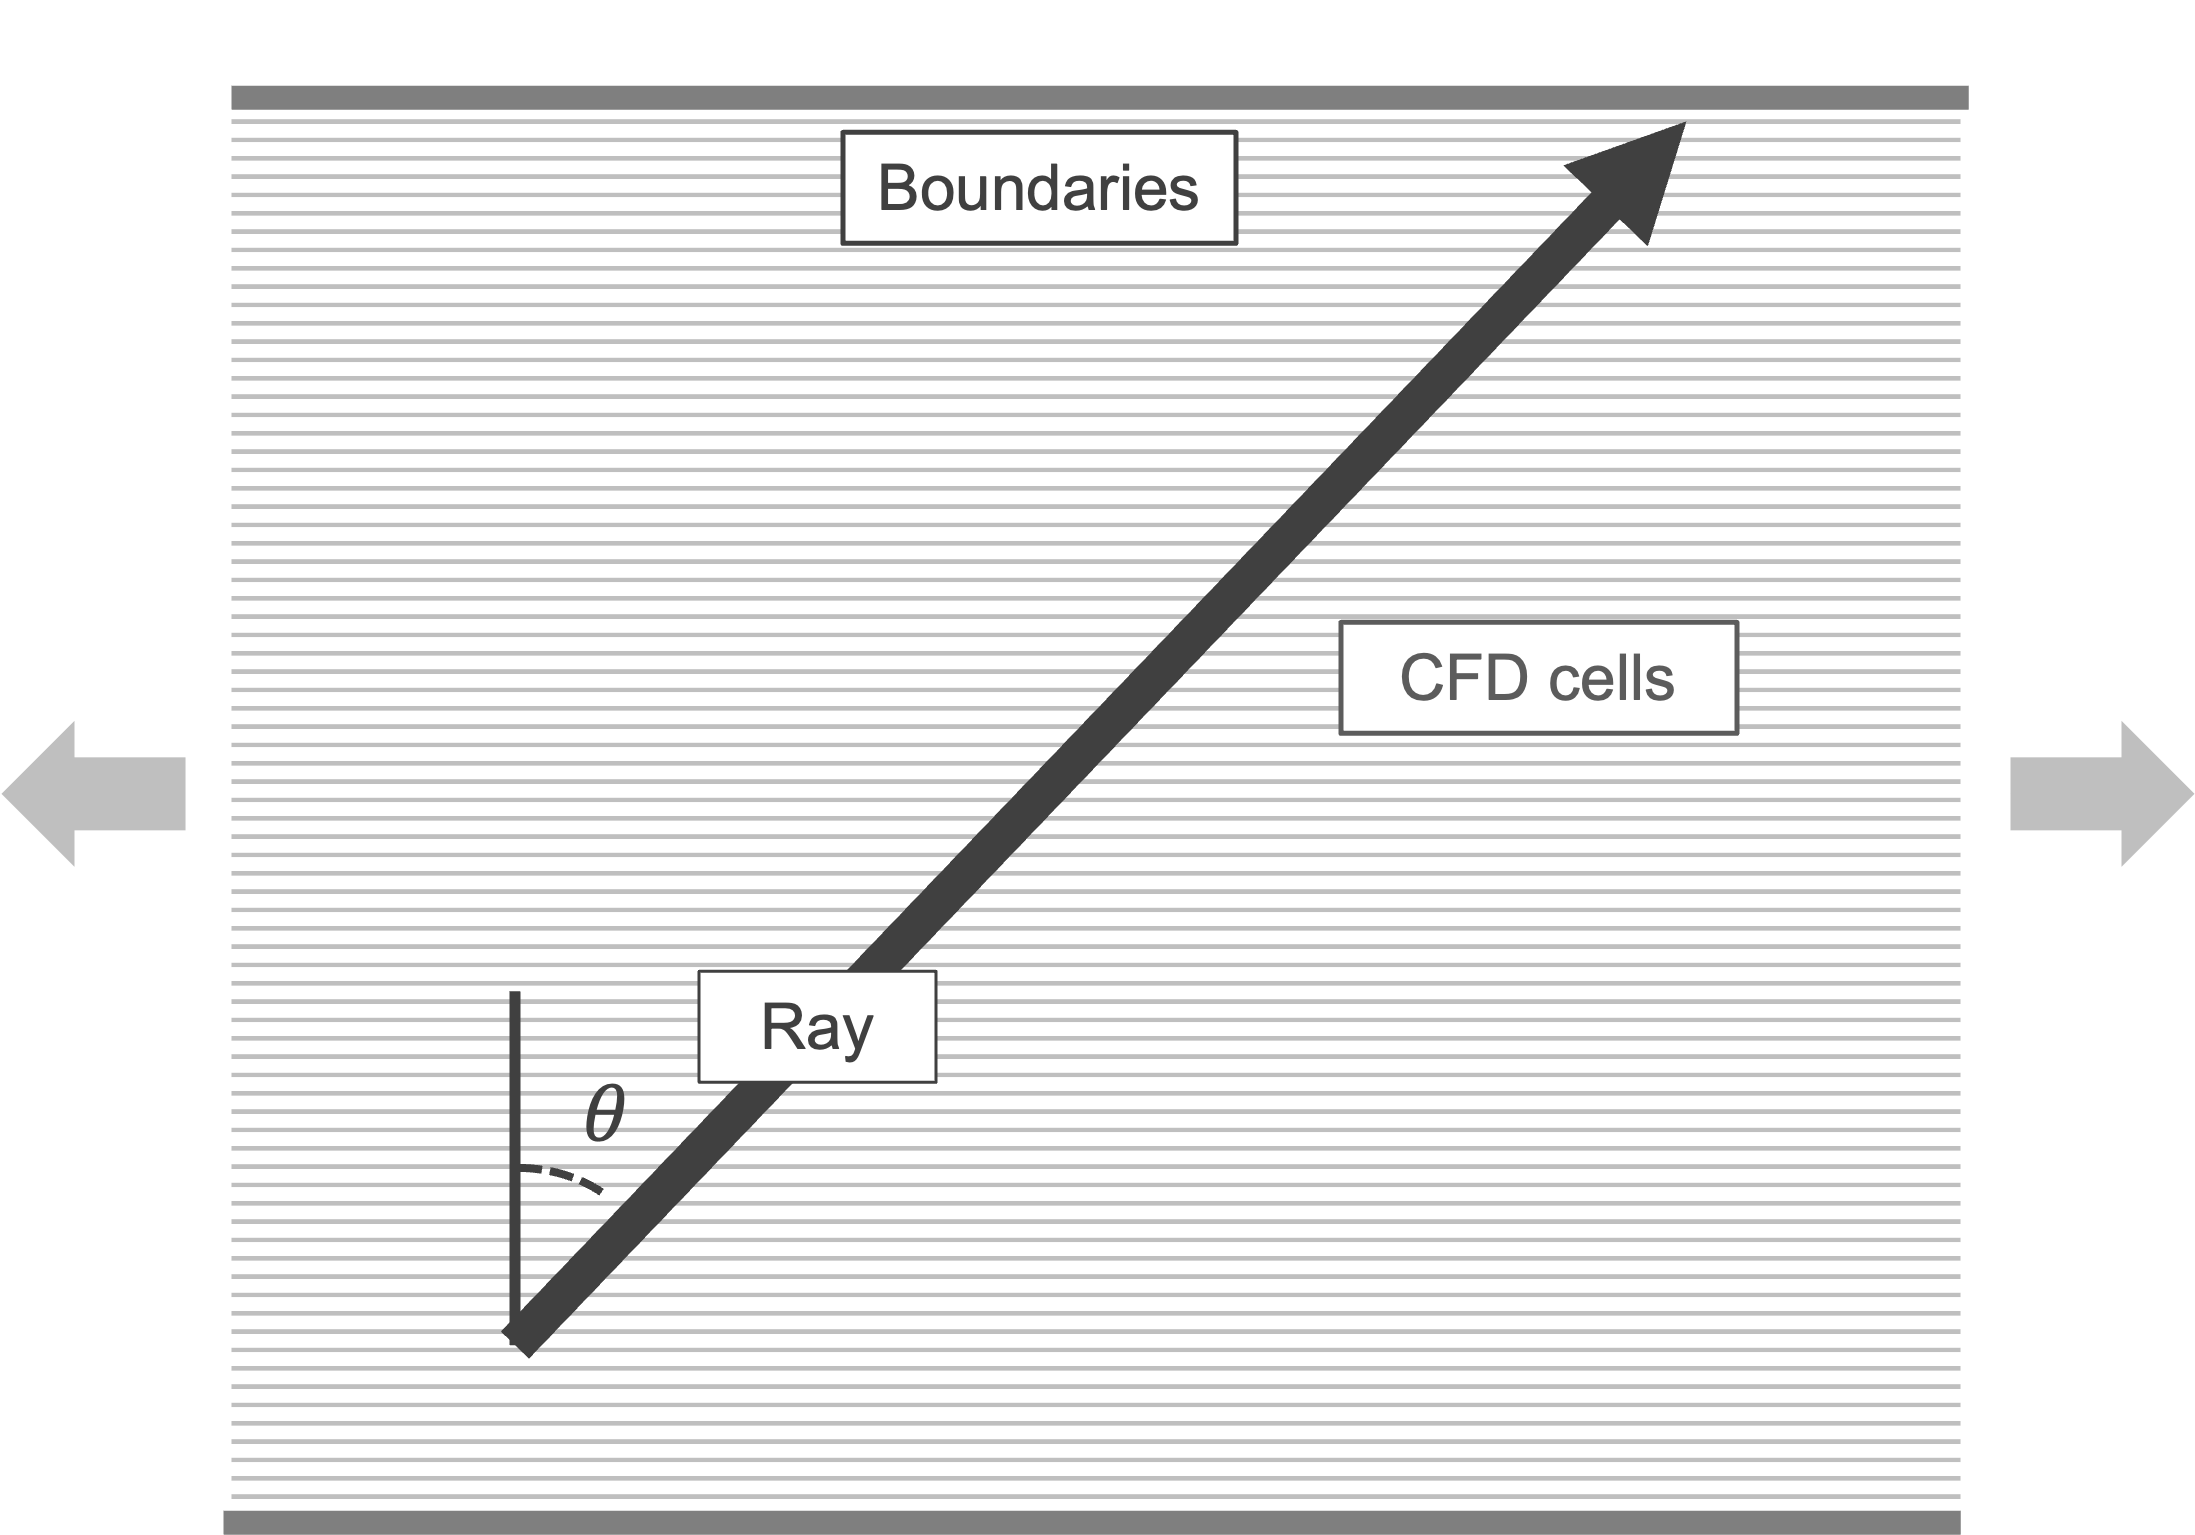
\includegraphics[width=0.5\linewidth]{figures/ch2/PlaneParallelVisualization.png}
\caption{Plane parallel medium. Reflective walls are marked in gray, cold-black walls are marked in blue. }
\label{fig:PlaneParallel}
\end{figure}

The modified RTE, Eq.~\ref{eq:RTErewritten}, is repeated below for convenience as 
\begin{equation}
    \frac{dI_\eta{}}{d\tau{}_\eta} = S(\tau_\eta,\hat{\textbf{s}})-I_\eta{} ~,
    \label{eq:RTErepeated}
\end{equation}
where $d\tau_\eta$ has been substituted for $\beta_\eta{}ds$, as discussed in section~\ref{section:RTE}. An integration factor $e^{-\tau_\eta}$ may be multiplied through as  
\begin{equation}
    e^{-\tau_\eta}\frac{dI_\eta{}}{d\tau{}_\eta} + e^{\tau_\eta}I_\eta= S(-\tau_\eta,\hat{\textbf{s}})e^{-\tau_\eta} ~,
\end{equation}
\begin{equation}
    \frac{dI_\eta{}e^{-\tau_\eta}}{d\tau{}_\eta} = S(\tau_\eta,\hat{\textbf{s}})e^{-\tau_\eta} \ .
\end{equation}
After integration, this becomes,
\begin{equation}
    I_\eta{}(\tau_\eta) = I_\eta{}(0)e^{-\tau_\eta} + \int_0^{\tau_\eta}{S(\tau_\eta',\hat{\textbf{s}})e^{-(\tau_\eta-\tau_\eta')}}d\tau_\eta' ~.
    \label{eq:RTEintegrated}
\end{equation}
The source term $S(\tau_\eta',\hat{\textbf{s}})$, is defined in Eq.~\ref{eq:RTE_S},
\begin{equation}
    S(\tau_\eta',\hat{\textbf{s}}) = (1-\omega{}_\eta{})I_{b\eta{}}+\frac{\omega{}_\eta{}}{4\pi}\int_{4\pi{}}{I_\eta{}(\hat{\textbf{s}})\Phi_\eta{}(\hat{\textbf{s}}_i,\hat{\textbf{s}})}\,d\Omega{}_i ~,
    \label{eq:RTE_S}
\end{equation}
where $\omega_\eta$ is the single-scatter albedo, $\omega_\eta=\sigma_\eta/(\sigma_\eta+\kappa_\eta)$. The first and second components of the source term describe the emission of radiation along $\hat{\textbf{s}}$ and the in-scattering of radiation into direction $\hat{\textbf{s}}$. Within a plane-parallel medium, properties only vary along the axis normal to the walls. Therefore, the coordinate $\tau{}_\eta{}$ may be transformed to a wall-perpendicular coordinate as $\tau{}_{p\eta{}}=\tau{}_\eta{}\cos{\theta}$, where $\theta$ is the angle between the ray direction and the perpendicular axis. Extending this transformation to Eq.~\ref{eq:RTEintegrated} results in
\begin{equation}
    I^+_\eta{}(\tau_{p\eta},\theta) = I_{1\eta{}}e^{-\tau_{p\eta}/\cos{\theta}} + \int_0^{\tau_{p\eta}}{S(\tau_{p\eta}',\theta)e^{-(\tau_{p\eta}-\tau_{p\eta}')/\cos{\theta}}}\frac{d\tau_{p\eta}}{\cos{\theta}}' \ ,
    \label{eq:RTEplus}
\end{equation}
and
\begin{equation}
    I^-_\eta{}(\tau_{p\eta},\theta) = I_{2\eta{}}e^{-(\tau_{Lp\theta}-\tau_{p\eta})/\cos{\theta}} + 
    \int_{\tau_{Lp\eta}}^{\tau_{p\eta}}{S(\tau_{p\eta}',\theta)e^{(\tau_{p\eta}-\tau_{p\eta}')/\cos{\theta}}}\frac{d\tau_{p\eta}}{\cos{\theta}}' \ .
    \label{eq:RTEminus}
\end{equation}
$I^+_\eta$ and $I^-_\eta$ are spectral intensities propagating in the positive and negative $\tau_{p}$ directions, respectively. Also, $I_{1\eta}$ and $I_{2\eta}$ are the emitted intensities from walls 1 and 2 at $\tau_{p\eta}=0$ and $\tau_{p\eta}=\tau_{Lp\eta}$, respectively. The split of Eq.~\ref{eq:RTEintegrated} into Eqs.~\ref{eq:RTEplus} and \ref{eq:RTEminus} is convenient by allowing the emission from each boundary to be individually accounted for. As a whole, Eq.~\ref{eq:RTEplus} represents the emission of radiative intensity from below the point of interest $\tau_{p\eta}$ (including the boundary at $\tau_{p\eta}=0$ with intensity $I_2{\eta}$) up to the point of interest, and Eq.~\ref{eq:RTEminus} represents the same but for above the point of interest.

With the solution for spectral radiative intensity obtained, the overall divergence of heat flux can also be evaluated by completely solving Eq.~\ref{eq:DivHeatFlux2}. The first term in Eq.~\ref{eq:DivHeatFlux2} can be calculated using the provided parameters for $\kappa_\eta$ and $I_{b\eta}$. The second term, which represents the absorption coefficient times \textit{irradiance} $G_\eta$ may be calculated as
\begin{equation}
    \centering
    G_\eta{}(\tau{}_{p\eta})=\int_{4\pi}I_\eta \, d\Omega{}
    =\int_0^{2\pi}{}\int_0^{\pi}I_\eta(\tau_{p\eta},\theta)\sin{\theta} \, d\theta{} \,d\psi{} \ ,
\end{equation}
\begin{equation}
    \centering
    G_\eta{}(\tau{}_{p\eta})=2\pi{}\int_{-1}^{+1}I(\tau{}_{p\eta},\mu) \,d\mu
\end{equation}
where $\mu=\cos{\theta}$. Splitting the intensity into positive and negative components results in
\begin{equation}
    \centering
    G_\eta{}(\tau{})=2\pi{}\left[\int_{-1}^0{} I^-(\tau_{p\eta},\mu)\, d\mu{} + 
    \int_{0}^{+1} I^+(\tau_{p\eta},\mu)\, d\mu{} \right]
\end{equation}
and substituting in the solutions for $I^+_\eta$ and $I^-_\eta$, Eqs.~\ref{eq:RTEplus} and \ref{eq:RTEminus}, leads to
% \begin{multline*}
%     \centering
%     G_\eta{}(\tau{}_{p\eta})= 2\pi{}\left[I_{b1\eta}E_2(\tau{}_{p\eta})
%     +I_{b2}E_2(\tau{}_{Lp\eta}-\tau{}_{p\eta})
%     +\int_0^\tau{}_{p\eta}I_b(\tau{}_{p\eta}')E_1(\tau{}_{p\eta}
%     -\tau{}_{p\eta}')d\tau{}_{p\eta}'\\
%     +\int^{\tau{}_{Lp\eta}}_{\tau{}_{p\eta}}I_b(\tau{}_{p\eta}')E_1(\tau{}_{p\eta}'
%     -\tau{}_{p\eta})d\tau{}_{p\eta}'\right]
% \end{multline*}
\begin{equation}
\begin{split}
    G_\eta{}(\tau{})&=2\pi{} \left[ I_{b1\eta}E_2(\tau{}_\eta{})+I_{b2\eta}E_2(\tau{}_{L\eta}-\tau{}_\eta{})+\int_0^{\tau{}_\eta{}}S(\tau_\eta')E_1(\tau_\eta-\tau_\eta')d\tau_\eta' \right. \\
    &\quad \left. {}+\int^{\tau{}_{L\eta}}_{\tau{}_\eta{}}S(\tau_\eta{}')E_1(\tau_\eta{}'-\tau_\eta)d\tau_\eta' \vphantom{\frac12}\right]
% a &= \left( \frac12 + \frac13 + \frac14 \right. \\
%   &\quad \left. {}+ a + b + c \vphantom{\frac12}\right)
    \label{eq:IrrPlaneParallel}
\end{split}
\end{equation}
\begin{equation}
    \centering
    E_n(x)=\int_0^1\mu{}^{n-2}e^{-x/\mu{}}d\mu{} \,
    \label{eq:ExpInt}
\end{equation}
where $I_{b1\eta}$ and $I_{b2\eta}$ are the spectral black body intensities from the two boundaries, the subscript $p$ has been removed, and $E_n$ is the exponential integral defined in eq. \ref{eq:ExpInt}. 

Equation~\ref{eq:IrrPlaneParallel} can be computationally expensive to solve in a scattering medium because the scattering component of $S(\tau{}_\eta')$ is also a function of $G_\eta(\tau_\eta)$, rendering Eq.~\ref{eq:IrrPlaneParallel} implicit. One numerical approach is to provide an initial guess irradiance field $G_\eta(\tau_\eta)$, evaluate $S(\tau{}_\eta')$, and integrate for another solution to $G_\eta(\tau_\eta)$. The process can be repeated until $G_\eta(\tau_\eta)$ has converged. Such a solution procedure is computationally inexpensive in a medium with little to no scattering, but can become expensive under high scattering.
Finally, provided a solution to $G_\eta{}(\tau_\eta)$, the spectral radiative absorption at every point may be evaluated as $\kappa{}_\eta{}G_\eta{}(\tau_\eta)$, and the overall volumetric radiation source term at any point can be evaluated as 
\begin{equation}
    \centering
    Q_{src}=\int_0^\infty{}\kappa{}_\eta{}G_\eta{}d\eta{}-4\kappa_p\sigma{}T^4 .
    \label{eq:RadSrcPP}
\end{equation}


\subsection{Frozen-Field Analysis}
The speed of light in a vacuum may be much higher than even the fastest processes within a combustion simulation. As such, the flow may be considered static during the traversal of a ray, and the solution of radiation for a timestep may be decoupled from the rest of the physics modeling.
A \textit{frozen-field analysis} is one approach used in many thermal radiation models. In frozen-field analysis, a single time-step of a Computational Fluid Dynamics (CFD) simulation is extracted, and a solution for the RTE is evaluated using a radiation model. 
This approach is convenient and less computationally expensive for testing a radiation solver because a full solution of radiation at every timestep from initial conditions is not required.

\section{Influences of radiation}
% The redistribution of thermal energy facilitated by radiation may effect a combustion system in a number of ways.
% combustion systems from both a physical and modeling perspective. A variety of these influences will be discussed in this section. 

% First, the direct influences on fluid-dynamics are presented, followed by influences specific to turbulent flows, to the enclosing walls or surrounding objects, and to the chemical propagation and product mixture compositions.

\subsection{Coupling to fluid dynamics}
There exists a strong coupling between radiation and fluid dynamics within many combustion systems. Redistribution of thermal energy results in changes to local thermodynamic states. This may lead to, for example, density changes that result in buoyant fluid motion. Furthermore, changes in fluid motion from external influences like wind may result in stymied combustion, which can lead to decreases in radiative emission~\cite{Hu2017AChallenges}.

A key area of study in radiating flames are wild-land fires. The large length scales and high degrees of emissive power from fires result in a significant, non-negligible influence of radiation within the flame and to the surroundings~\cite{Drysdale2011AnDynamics}. If surrounding objects are flammable, then radiation can ignite new flames at a distance resulting in increased fire spread and damage~\cite{Valendik2008EffectEnvironment}. Extensive research has been conducted in determining the exact contribution of radiation in these flames~\cite{Sacadura2005RadiativeScience} in order develop preventative methods to inhibit flame radiation such as water droplets~\cite{Wu2018RadiationStudy}. 
Recent technological advances have seen improvements in modeling and diagnostic methods, resulting in more informed computational and experimental findings, but many fundamental questions on the contributions of radiation to the flame and fluid dynamics remain to be answered~\cite{Finney2013OnSpread}. Broadly speaking, it is known the coupling of radiation to momentum fields largely take place over long length and time scales~\cite{Tieszen2001ONFIRES}. Turbulent puffing motions and toroidal vortices resulting from buoyant and baroclinic forces~\cite{Cetegen1993ExperimentsFires} may result in changes in soot production~\cite{Chen2023PoolAdvances}. Soot is often a primary radiator from many hydrocarbon flames, amounting to 25 to 35\% energy escaping~\cite{Tieszen2001ONFIRES}. However, high concentrations of soot surrounding a large flame may also block radiation to the surroundings~\cite{Hamins1995CharacteristicsBurning}. Evidence largely supports that larger fires have more significant contribution of radiation~\cite{Chen2023PoolAdvances}. However, \citet{Hiroshi1988AirFires} experimentally tested flames ranging from $0.3$ and $6$ meters in diameter and determined the soot radiation blocking effect appeared in sizes $2$ meters and above.


Pool-fires are the most common type of fire scenario that occurs in chemical process industries~\cite{Miao2014AccidentDike} and are also a common surrogate used to experimentally and computationally model many other kinds of real fires~\cite{Chen2023PoolAdvances}. A pool fire is a canonical configuration where a liquid pool of fuel is vaporized, ignited, and reacts with surrounding oxidizer. Much research has been conducted using this configuration to determine the influence of turbulent fluid motion, wind, and flow structures on radiative heat flux and vice versa~\cite{Chen2023PoolAdvances}.
For example,~\citet{Hu2017AChallenges} discussed the influences of flame tilt to the view-angle of a flame to a boundary. When a powerful gust of wind tilts the flame, less of the flame is visible to an adjacent object, resulting in reduced radiation. This effect results in a decrease of the incident heat flux, and therefore vaporization rate, of the pool, and can therefore limit the fuel supply and have a concomitant influence on all characteristics of the flame.

In general, radiation is a `dissapative process'. As a result, redistribution of thermal energy may lead to a reduction in local turbulence intensity~\cite{Modest2016RadiativeSystems}. \citet{Li2002InvestigationMethod.} studied the influence of radiation in scaled flames and determined increasing radiation resulted in considerable decreases in temperature fluctuation. \citet{Wang2008MonteFlames} calculated radiation reductions of 5\% in their artificially scaled Sandia D flames. \citet{Consalvi2012InfluenceFires} presented reductions approaching 10\% in simulations with radiation compared to those without. In all, the exact influences of radiation on turbulence are masked due to computational expense and lack of adequate turbulence/radiation interaction (TRI) modeling to accounting for the non-linear influence of unresolved turbulent fluctuations in LES and RANS simulations~\cite{Modest2016RadiativeSystems}.

% Pool-fires: buoyancy drive dynamical influences of flames. Leads to significant contribution to teh spread of fires??

% Many fluid dynamic systems see a relevant contribution of radiation. These physics that are present with non-chemically reacting flows can present themselves equally or in greater magnitude in reacting flows, and therefore provide a useful initial basis to define the influence of radiation in combustion. 
% To a degree, any gas-dynamical system with high temperatures and relatively low densities will exhibit high degrees of radiative emission compared to conduction and convection~\cite{Pai1966RadiationDynamics}. This includes the fields of hypersonics, fission and fusion nuclear energy, and space exploration.

% For many non-chemically reacting systems, the gasdynamical influences of radiation take effect often in regimes of science well-beyond those seen in every day life. Under atmospheric conditions, for example, the influence of radiation is largely negligible compared to that of conduction and convection \cite{Pai1966RadiationDynamics}.
% Even under hypersonic conditions, such as inter-continental ballistic missiles (ICBMs), radiation is often still an order of magnitude lower than aerodynamic heating. Only at temperatures seen by re-entry vehicles (10$^4$ K) does radiation have a strong, non-negligible effect.
% In nuclear systems, such as nuclear fusion reactors, where temperatures reach 10$^6$K, the influence of the radiation becomes extremely significant. This follows from not only its redistribution of energy, but also its influence on pressure (through momentum imparted via photon collisions) and the radiative energy density become non-negligible as well. 

% In fluid dynamics, there is often the coupled contribution of radiation to the buoyancy.
% Additionally, in conditions of long residence times, radiation has a longer time to impart a reduction in energy to the fluids present in the system. This may result in 

% Buoyancy effects
% Microgravity effects
% Dr. Zhaos paper




\subsection{Radiation in enclosed engines}
Relatively few studies have focused specifically on the contribution of radiative heat transfer to the boundaries of enclosed combustion engine systems. Most existing models involve low-fidelity gray models combined with inaccurate radiation solvers, such as P-1. A brief review of existing research of radiation to the boundaries of gas-turbine engines and rocket engines is first provided, followed by a review of radiation modeling within surrounding protective thermal barrier coatings.

\subsubsection{Radiation incident on the boundaries}

Modern gas-turbine combustors operate at temperatures that far exceed the material limits of the enclosing materials~\cite{Padture2016AdvancedPropulsion}.
These extreme conditions pose a risk of harmful wear and damage to the combustion chamber or downstream turbine stages. Advanced cooling techniques are employed such as film cooling to mitigate the damaging and potentially dangerous effects of these conditions~\cite{Amano2008ThermalSystems}. However, excessive cooling for material protection may present a significant thermodynamic loss to the system, reducing the overall work contribution from the energy conversion process.
As a result, an understanding of the influence of all modes of heat transfer along the boundaries has seen increased importance.

\citet{Lefebvre1984FlameChambers} provided an early review on radiation in gas-turbine chambers. Radiative emission is known to contribute significantly to wall heat flux, in particular for high pressure and highly luminous flames. Also, the challenge of predicting radiative emission and absorption rates while accounting for soot formation, non-gray modeling, and other variables were described. \citet{Claus1981SpectralCombustor} conducted an experimental study of radiation from a Pratt \& Whitney JT8D tubular can combustor and found that soot contributed 70–80\% of radiative emission in the primary zone, 50-70\% in the intermediate zone, and 35–50\% in the dilution zone.
\citet{Berger2016OnLoads} conducted time-accurate simulations of a helicopter engine combustor to compare the influences of conjugate convection and radiation on the system boundaries. They applied the Discrete Ordinates Method (DOM), a relatively low-cost radiation model with high accuracy, combined with a statistical narrow-band non-gray model accounting for CO$_2$, CO, and H$_2$O, and a large-eddy simulation with the thickened-flame approach for chemistry modeling. Their results showed convection and radiation contributed similar orders of magnitude to wall heat fluxes, with radiation primarily contributing heat to the colder-wall regions and reducing flame temperatures. Radiative energy was shown to contribute a neglegible difference to the thermodynamics of the flame, contributing two orders of magnitude less energy than the chemical heat release. Finally, good agreement was obtained to experimental results. 
\citet{Paul2006RadiativeCombustor} applied the DOM to a CFD simulation of the Rolls Royce Tay gas turbine geometry. Soot and non-gray absorption were neglected. Emission was shown to maximize in regions where temperature is maximized. However, the authors noted the contribution of soot may effect these results.
\citet{Gamil2020AssessmentChamber} compared the contribution of radiation in a Rolls-Royce RB-183 turbofan engine combustor using the DOM and the P-1 approximation, another radiation model. The influences of soot and non-gray absorption were again neglected.
The combustor geometry follows a Rich-Quenched-Lean (RQL) design, where a high temperature, non-premixed flame is followed by a high degree of mixing with dilution gases, which is followed by a premixed fuel-lean reaction to the aft section of the combustor.
Apparently, radiation resulted in a 10\% higher temperature in the liner near the fuel-rich zone, and a 15\% reduction of temperature after the dilution zone.
In total, radiation was shown to reduce peak flame temperatures by 200K compared to with no radiation for their time-accurate simulation.
The P-1 model was shown to over-exaggerate the effect of radiation compared to the more accurate DOM.
\citet{Ghose2016PredictionLevels} conducted similar time-accurate simulations of a mock gas-turbine combustor using the DOM radiation method with a weighted-sum of gray gases non-gray model and an empirical correlation for soot. They observed that radiation exhibited significant control over the incident heat flux to the injector and combustor walls, and soot played a significant role in emission. They also observed a strong dependence of radiation on the geometry: where increasing injector swirl resulted in an axially tightened flame with lower peak radiative heat flux to the walls.



Radiation has also been shown to contribute significantly in rocket engines. Between 5\% and 30\% of the overall heat flux at the walls can be attributed to emission from the medium \cite{Johnson2021AnalysisMethod,Sutton2001RocketElements,Naraghi2005ModelingEngines,Pizzarelli2021OverviewChambers}. \citet{Leccese2018ConvectiveChambers} evaluated the influence of radiation and convection using a RANS CFD model with gray-gas radiation. 
They observed radiation contributions totaling to 15\% and 11\% for liquid methane/liquid oxygen and liquid hydrogen/liquid oxygen, respectively.
\citet{Leccese2019NumericalChambers} later studied the influences of radiation in a Space Shuttle Main Engine (SSME) in a time-accurate simulation, but with no radiative contribution to the energy equation.
They observed peak wall-incident radiative heat flux follows where peak temperatures occur, within the combustion chamber rather than the throat or nozzle. They also developed a resource to gather predictions of wall heat transfer coefficients and fractional contributions of radiation as a function of chamber pressure and diameter for both liquid methane/liquid oxygen and liquid hydrogen/liquid oxygen.
Radiative contribution was shown to increase with a decrease in pressure and an increase in chamber diameter.

Additional studies have shown that radiation plays a very significant role in the wall heat fluxes in heavy-duty diesel pistons, re-entry vehicles, and many combustion technologies of recent interest such as oxy-fuel combustion \cite{Modest2016RadiativeSystems,Viskanta1987RadiationSystems}.


\subsubsection{Thermal Barrier Coatings}
In many systems, the high temperatures associated with combustion may exceed the melting points of the materials of the outer casing~\cite{Flamant2019OpportunitiesCoatings}. This can potentially be a limiting factor to consider during the design of these systems, such as in a gas-turbine combustor.
A Thermal Barrier Coating (TBC) is a protective ceramic coating often applied to the interior walls of combustion systems to manage the heat loads to the outer surfaces. 
TBCs are usually constructed from a specialized Zirconia ceramic, which has the capability to resist heat
better than most materials~\cite{Miller1997ThermalDirections}. Specifically, Yttria-stabilized zirconia (YSZ) provides adequate performance for modern TBCs~\cite{Padture2002ThermalApplications,Padture2016AdvancedPropulsion}. At high temperatures, these materials become transparent to most thermal radiation, and the resulting heat transfer analysis becomes more complex~\cite{Howell2010ThermalTransfer, Siegel1998AnalysisCoatings} because radiative heat transfer plays a more significant role within the mechanism. The
introduction of gas-filled pores also induces ray scattering, which has been shown to reduce metal temperatures~\cite{Boissonnet2019EvolutionTemperature,Spuckler1996Two-FluxLayers}, but further complicates the understanding of the system.

Analysis between the flame, TBC, metal, and cooling impingement flow includes all three forms of heat
transfer: conduction, convection and radiation. Conjugate modeling of the three forms can be computationally intensive, especially when using exact methods~\cite{Viskanta1975HeatSolids}. 
The inclusion of radiative heat transfer within the conjugate heat transfer model makes a solution analytically intractable when complex material properties and boundary conditions are involved.
As a result, appropriate modeling of TBCs is rare in high temperature systems. A fully comprehensive, one dimensional, analytical method was presented by~\citet{Siegel1996InternalCoatings}. Through the use of the Milne-Eddington approximation for radiation, the method can solve conduction and radiation simultaneously
within the semitransparent TBC \cite{Milne1930ThermodynamicsStars,Eddington1920TheStars}. The TBC is assumed to have a cutoff wavelength, $\lambda{}_c$ where all incident radiation of wavelength below $\lambda{}_c$ passes through the TBC surface and is solved according to the RTE. All remaining incident radiation is absorbed at the surface and modeled within the TBC as conductive diffusion~\cite{Yang2013ExperimentalCoatings}.
The combined heat transfer solution for the TBC was established to be very accurate in most circumstances and not very computationally expensive according to~\citet{Siegel1996InternalCoatings}. 
However, assumptions such as gray gases, one-dimensionality, and two flux can limit the applicability of Siegel’s method. \citet{Johnson2021AnalysisMethod} coupled the Siegel’s method with a Monte Carlo ray tracing analysis of a gas turbine combustor, where non-gray radiation from the flame is accounted for. Differences in temperature as large as $150$ K were observed within the TBC between non-gray and gray analyses.
Finally,~\citet{Tricard2021ModelingEnvironments.} generated a 3-D model of conjugate heat transfer in a semitransparent TBC at steady state using MCRT radiation coupled with Finite-Volume Method (FVM) conduction. 
The simulation followed that of~\citet{Siegel1996InternalCoatings}, where a cutoff wavelength was assumed.
Results where comparable to Siegel's method, and three dimensional influences were shown to be influential to the steady-state temperature distribution in the domain. Additionally, a parametric study concluded that increasing $\lambda{}_c$ results in a decrease in peak temperature and a trend of decreasing heat flux through the TBC as a result of increased net reflectance of heat.
\begin{figure}
\centering
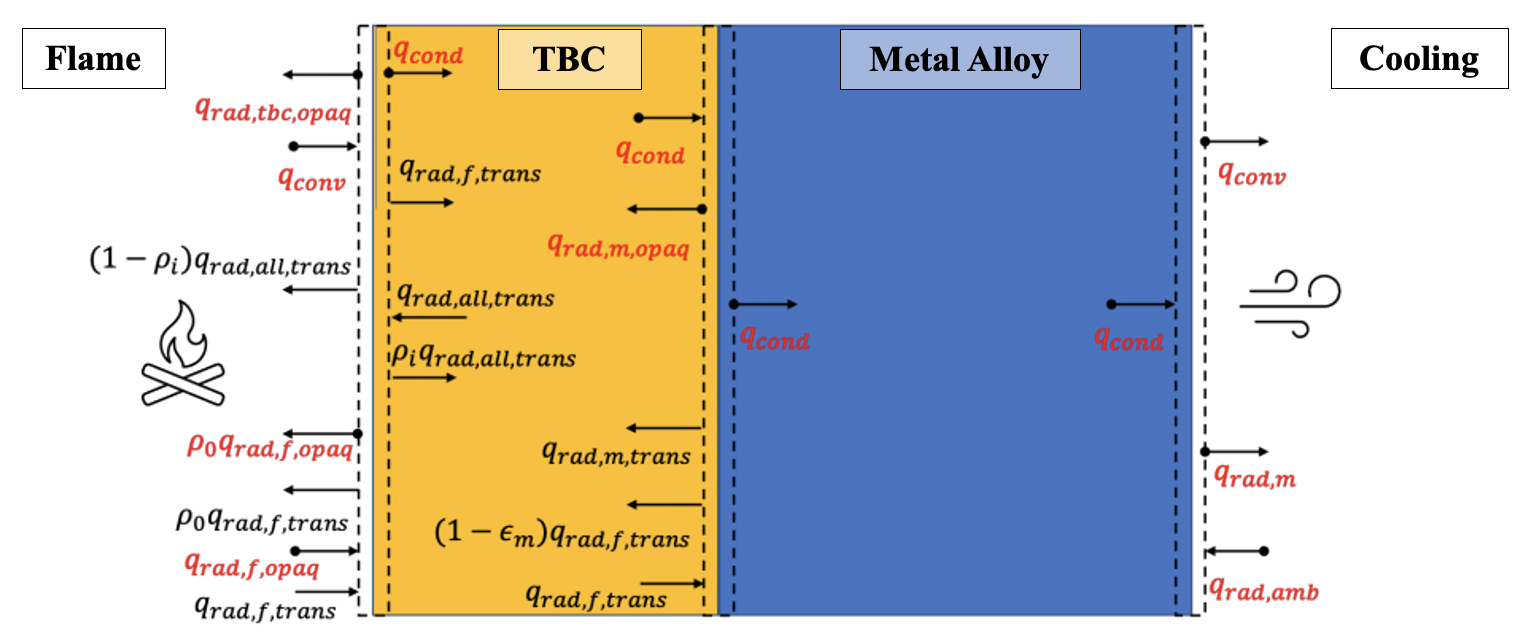
\includegraphics[width=1\linewidth]{figures/ch2/TBC.png}
\caption{The computational domain for the conjugate heat transfer solver from~\cite{Tricard2021ModelingEnvironments.}. Various sources of heat transfer rate are labeled, with the red-fonted heat transfer rates accounted for by the conduction solver and the black-fonted heat transfer rates accounted for by the radiation solver. The yellow domain and blue domains are the TBC and metal, respectively. The x direction follows from the flame to the impingement flow. The y and z directions are vertical and into the page, respectively. }
\label{fig:TBC}
\end{figure}

\subsection{Changes to chemistry}
The physics of combustion processes are often highly dependent on the accompanying chemical reaction network.
The multitude of reactions that proceed during the conversion from the reactant molecules to the product species in combination with changes to the existing macroscopic thermodynamic properties results in a complex modeling procedure.
For one, radiation has been shown to influence the temperature of a system. Temperature has a high degree of control on the chemical reaction rates of combustion.
This presents an additional, indirect, influence of radiation on the chemical process, one that requires coupled modeling of thermal, fluid, and chemical processes within a combustion simulation for an adequate analysis.

\subsubsection{Extinction and Flame Speed}
Characterizing the extinction limits of a flame is a useful measure for many applications. Radiation has been a known contributor the lean flammability limits of many flames~\cite{Ju2000AsymptoticFlames,Liu2020TheFlames}.
Many one-dimensional simulations and experiments have been performed for the purpose of investigating this phenomenon.
\citet{Lakshmisha1991OnChemistry} simulated one-dimensional CH$_4$/air flames with the OTA radiation model near lean flammability limits. They demonstrated that radiant heat loss is the primary cause of flame extinction when the lean flammability limit is approached.
\citet{Ju1998EffectsFlames} investigated the influence of radiation absorption within a premixed flame.
They determined that accounting for radiation re-absorption can lead to wider extinction limits and higher burning velocities. Further, the optically thin assumption leads to significant decreases in product species temperatures, while absorption will retain product temperatures and additionally allow for pre-heating of the reactants.
Additionally, through the use of a statistical narrow-band model, the influences of non-gray emission patterns lead to a significant escape of radiation through the reactant zone. They observed the difference in the emission spectrum from high temperature CO$_2$ and absorption spectrum of the low temperature CO$_2$ supplied along with reactants can lead to a significant escape of energy upstream of the flame. And they observed a similar trend for H$_2$O, where no H$_2$O was readily available in the reactants for absorption.

\subsubsection{Pollutant formation}
As discussed previously, radiation carries a strong influence on the temperature of combustion systems. 
And because temperature and chemistry are coupled, radiation also influences the product species concentrations at the exit of many combustion systems. In particular, the production of pollutant species NO$_x$ (nitrous oxides) and soot can be significantly affected \cite{Viskanta2010RadiativeSystems}.
\citet{Medwell2011TheRadiation} experimentally measured the influence of radiation in a laminar ethylene flame irradiated by a CO$_2$ laser. High incident radiation was shown to increase peak soot volume fraction by $250$\%, suggesting there exists a strong correlation of soot production with radiation.
\citet{Ihme2008ModelingFormulation} demonstrated the influence of radiation on NO$_x$ production by including an additional dimension to the flamelet progress variable approach for chemistry tabulation.
They applied the optically thin assumption (OTA) to simulations of the Sandia D. flame and the Pratt \& Whitney PW6000 combustor.
For both cases, production of nitric oxide was reduced by more than $60$\% compared to simulations without radiation included as a result of the lower peak temperatures. \citet{Ren2017MonteChamber} calculated the change in NOx output resulting from radiative emission within a gas-turbine combustion chamber. They determined that radiation modeled with line-by-line Monte-Carlo enhanced re-absorption in the flame and enhanced NOx emissions by almost $20$\% compared to combustors modeled without radiation.
\citet{Wu2021LimitationsFires} later highlighted the importance of including radiative absorption in these simulations using a budget analysis of relative contributions of various physics on temperature. 
They used mixture fraction ($Z$), a quantity to quantify the mixing between fuel ($Z=1$) and oxidizer ($Z=0$), to demonstrate the range of contributions of emission and absorption.
It was shown that radiative emission is very high near the stoichiometric mixture fraction, but decreases quickly around the fuel-rich and fuel-lean sides of the flame. Radiative absorption, in contrast, retains its magnitude across the mixture fraction range.
Additionally, to reduce the computational intensity of joint combustion-radiation calculations, they developed a cylindrical flamelet model to pre-tabulate the contribution of radiation to the pool-fire simulation with promising results.

